\subsection{Caso d'uso UC3: Login}
\begin{center}
	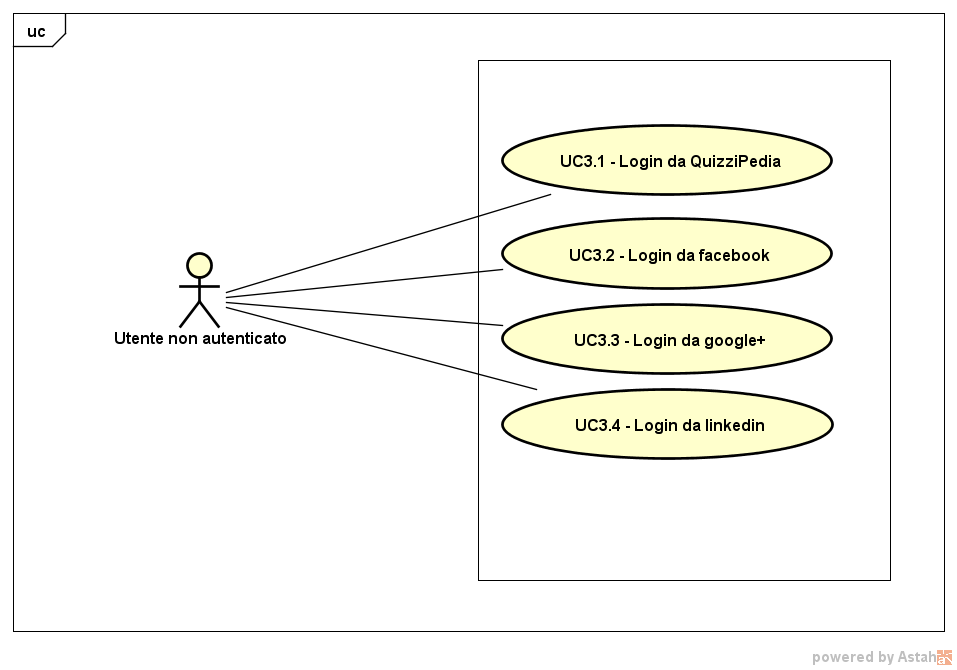
\includegraphics[scale=0.5]{UML/UC3.png}
\end{center}
\begin{itemize}
	\item \textbf{Attori:} Utente;
	\item \textbf{Scopo e descrizione:} l'utente si deve autenticare: inserisce nome utente e password con cui è registrato ed effettua il login;
	\item \textbf{Pre-condizione:} il sistema è avviato e pronto per l'utilizzo e mostra la pagina di login;
	\item \textbf{Flusso principale degli eventi:}
	\begin{enumerate}
		\item L'utente inserisce il nome utente oppure la mail utilizzata al momento della registrazione [UC3.1];
		\item L'utente inserisce la password [UC3.2];
		\item L'utente conferma il login[UC3.3].
	\end{enumerate}
	\item \textbf{Scenatio alternativo:}
	\begin{itemize}
		\item L'utente inserisce un nome utente inesistente;
		\item L'utente inserisce una mail non registrata;
		\item L'utente non inserisce ne un nome utente ne una mail;
		\item L'utente inserisce una password errata;
		\item L'utente non inserisce una password.
	\end{itemize}
	In tal caso il sistema ritorna allo stato precedente l'inserimento dei dati e viene visualizzato un messaggio d' errore.
	\item \textbf{Estensione:} l'utente visualizza un messaggio d'errore di autenticazione [UCD3.4].
	\item \textbf{Post-condizione:} il sistema ha autenticato l'utente e quindi mostra all'utente autenticato la sua area riservata.
\end{itemize}

\subsubsection{Caso d'uso UC3.1: inserimento del nome utente o della mail}
\begin{itemize}
	\item \textbf{Attori}: utente;
	\item \textbf{Scopo e descrizione}: l'utente inserisce il proprio nome utente creato oppure la mail utilizzata al momento della registrazione [UC2];
	\item \textbf{Precondizione}: il sistema presente all'utente lo spazio destinato a questa operazione;
	\item \textbf{Postcondizione}: il nome utente è stato inserito.
\end{itemize}
\subsubsection{Caso d'uso UC3.2: inserimento della password}
\begin{itemize}
	\item \textbf{Attori}: utente;
	\item \textbf{Scopo e descrizione}: l'utente inserisce la propria password associata al proprio nome utente creata al momento della registrazione [UC2];
	\item \textbf{Precondizione}: il sistema presenta all'utente lo spazio destinato a questa operazione;
	\item \textbf{Postcondizione}: la password associata al nome utente è stata inserita.
\end{itemize}
\subsubsection{Caso d'uso UC3.3: conferma login}
\begin{itemize}
	\item \textbf{Attori}: utente;
	\item \textbf{Scopo e descrizione}: l'utente conferma i dati inseriti per tentare una login;
	\item \textbf{Precondizione}: il nome utente o la mail e la password devono essere stati inseriti;
	\item \textbf{Postcondizione}: l'utente è autenticato.
\end{itemize}